\section{Empirical evaluation}
\label{sec:caseStudy}

%In this section, we perform an extensive empirical study evaluating the proposed energy procurement system.
% We first illustrate the fast convergence of SGA to the optimal
% solution in Figure~\ref{fig:convergence}. Then we continue to
% highlight the cost savings by using our system in Figure
% \ref{fig:cost_comparison}. The impacts of renewable energy
% penetration level and prediction errors are also studied.

\textbf{Experimental Setup.} There are 14 data centers in our system. They are located in 10
different states known to have Google data centers: California,
Washington, Oregon, Illinois, Georgia, Virginia, Texas, Florida, North
Carolina, and South Carolina. We merged the data centers in each state
creating 10 logical data centers in our simulation, i.e., $|N|=10$. We
assume that there are one million servers distributed across the ten
logical data centers, which is around half of the
number of servers in Amazon Web Services (AWS)
{\cite{AWSServers}}. The peak power consumption for each server is
300W.
%We set the other parameters based on the baseline case of using the nearest routing technique where the workload is just forwarded to the nearest data centers. 
We consider 40 sources, corresponding to 40 states of the US; the
corresponding workload data is obtained from Akamai Technologies. We
use the model \eqref{eq:delaycost} for capturing the monetary cost of
delay. The average workload is 30\% of the total capacity of the data
centers. The network delays $\pi_{ij}$ are estimated to be
proportional to the distance between sources and data centers
\cite{ATTNetworkLatency}. The average network delay is $22$ ms.
% The average queueing delay is $14.2$ ms. \jk{How do we arrive at
% this number? Does the queueing delay not depend on the algorithm?}
The parameter $\beta$ is estimated according to the fact that 100
ms latency costs 1\% of Amazon in sales \cite{liddle2008amazon}.



To compute the energy costs of the system, we assume that the system
purchases energy in long-term markets and real-time markets for an
hour of operation. The electricity prices in real-time markets are the
industrial electricity prices of each state in May 2010
\cite{eia2015}. Specifically, the mean values of real-time electricity
prices, $\mathbb{E}[p^r_i]$, of the considered states (in cents per
kWh) are as follows: 10.41 in California, 3.73 in Washington, 5.87 in
Oregon, 7.48 in Illinois, 5.86 in Georgia, 6.67 in Virginia 6.44 in
Texas, 8.60 in Florida, 6.03 in North Carolina, and 5.49 in South
Carolina. Since electricity prices in long-term markets are usually
much cheaper than that of the real-time markets, we set the long-term
prices such that the ratio $\frac{\mathbb{E}[p^r_i]}{p^l_i }=2.5$ for
all results, except for Figure~\ref{fig:prices}, where the ratio is
varied.
%We set $\beta$ = 1 throughout the section except Figure
%\ref{fig:betas} where it varies. 


To simulate the uncertainties, the error distributions between 12-13
pm shown in Figure \ref{fig:hourlyDistribution} are used to generate
the samples of renewable energy generation (PV generation and/or wind
generation), workload, and electricity price. The mean absolute errors
(MAE) of prediction errors for PV generation, wind generation,
electricity price, and workload demand are $45\%$, $65\%$, $40\%$, and
$35\%$, respectively. The MAE are varied later to study the impacts of
prediction errors. Wind generation is used as the renewable energy
source by default. The penetration of the renewable energy is fixed at
$50\%$ of the averaged demand. We also vary the penetration of PV and
wind generation to investigate the impacts of the renewable portfolio
and penetration level.

\begin{figure}[!t]
	\centering
	\vspace{-0.2cm}
	\subfloat[Gradient components]{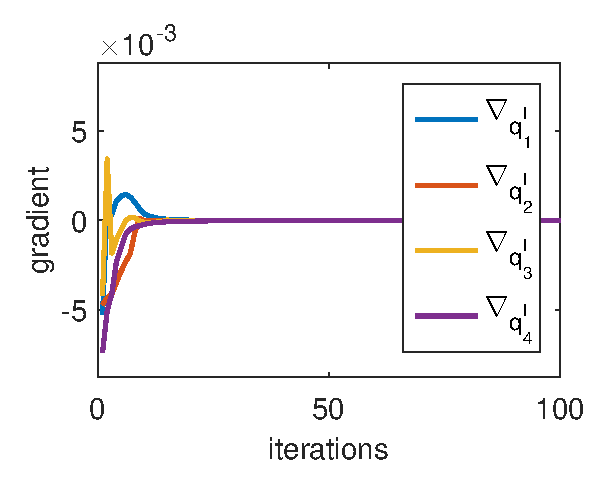
\includegraphics[width=.5\linewidth]{figs/grad_converge}}
	\subfloat[Long-term objective]{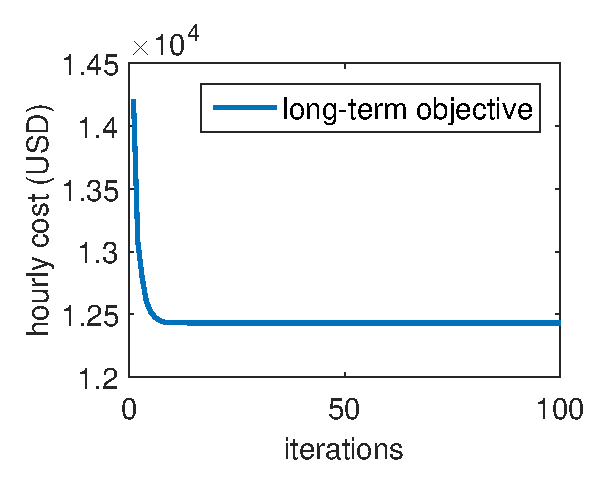
\includegraphics[width=.5\linewidth]{figs/obj_converge}}
	\vspace{-0.2cm}
	\caption{Convergence analysis.}
	\label{fig:convergence}
	\vspace{-0.6cm}
\end{figure}

\textbf{Convergence of SGA.} Although SGA is proved to eventually
converge to the optimal value of EP-LT, the convergence can be slow in
practice. The convergence speed mainly depends on how the step sizes
are set. Stochastic approximation is known to have high computational
complexity due to the large numbers of iterations and samples needed
for each iteration. To reduce the number of iterations, we use the
step size update rule as $\eta_t=\frac{s}{(S+t+1)^\alpha},$ where
$s$ and $S$ are non-negative constants and $ 0.5 < \alpha \leq
1$. This form fulfills the requirement of
Assumption~\ref{ass:stepsize}.
% In general, larger $s$ can enhance the performance in the later
% iterations, but it may cause instability in the early
% iterations. Thus, $S$ is used to prevent the instability.
%% JK: Not sure if this much detail is needed.
To speed up the convergence of algorithm, each gradient component has
its own step-size, and the step-size is updated only if the gradient
component switches from negative to positive or vice versa. Figure
\ref{fig:convergence} illustrates four gradient components (of total
ten) and the long-term objective function updated over iterations. As
shown in the figure, gradient components, and the long-term objective
$F^l(q^l)$ converge very quickly, i.e it is very close to the optimal
value after merely 20 iterations. In general, some gradient components
$\nabla_{q^l_i}$ may converge to positive values. In such cases, the
optimal solution has $q^l_i=0$.

\textbf{Cost savings.} We highlight the benefit of our proposed system
by comparing with the following algorithms.

\textit{No long-term procurement or geographical load balancing (nLTnGLB)}: nLTnGLB does not participate in long-term markets, i.e. $q^l_i = 0$, $\forall i \in N$, and the workload demand are forwarded to the closest data centers, a.k.a., the nearest routing method. We assume that the data centers activate all servers to minimize the queueing delay, i.e. $m_i=M_i$. Though simple, this policy is still widely used in practice.

\textit{Fixed long-term procurement without geographical load balancing (fLTnGLB)}: Cloud providers purchase a fixed amount of electricity ahead. We assume that the long-term procurement is 50\% of workload mean. Like nLTnGLB, it uses the nearest routing method instead of GLB-RT.

\textit{No long-term procurement but with geographical load balancing (nLT)}: In this algorithm, cloud providers do not purchase the energy in long-term markets like nLTnGLB. However, they execute GLB-RT to minimize the total cost in real-time.

\textit{Fixed long-term procurement geographical load balancing (fLT)}: fLT buys a fixed amount of electricity in long-term markets same as fLTnGLB, i.e., 50\% of workload mean. In real-time markets, it executes GLB-RT.

In addition to the baseline algorithms, we compare our algorithms to \textit{Oracle Algorithm (OA)}. OA is an unrealizable algorithm that is given to the absolute performance limit by assuming assumes all realizations of renewable energy, workload, and electricity prices are fully known apriori. Similarly to PA, the problem of long-term procurement can then be solved efficiently. The cost of OA is measured by averaging its output over many realizations.

\desc{The benefits of the proposed system}

\begin{figure}[!ht]    
	\centering
	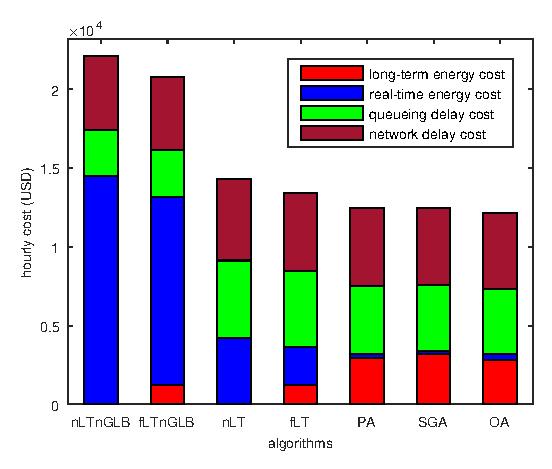
\includegraphics[width=.95\linewidth]{figs/cost_comparison}
	\vspace{-0.3cm}
	\caption{Cost comparison when $\beta=1$ and 50 \% renewable penetration. The proposed algorithms PA and SGA  are very close to the lower bound, OA and outperform the traditional methods up to 44\%.}
	\label{fig:cost_comparison}
	\vspace{-0.5cm}
\end{figure}

Figure \ref{fig:cost_comparison} compares the cost performance among our proposed algorithms and the traditional algorithms. The figure highlights that our proposed algorithms PA and SGA save up to 44\% compared to other simpler algorithms, and are comparable to the oracle algorithm (OA), the impractical lower bound. It also shows the significant benefits for cloud providers to participate long-term markets. Surprisingly, the performance of PA is very close to that of the SGA.

%\todo{read the paper A Control Theorist’s Perspective on Dynamic Competitive Equilibria in Electricity Markets by Wang et al. to see whether it can explain this observation.}

%\new{A Control Theorist’s Perspective on Dynamic Competitive Equilibria in Electricity Markets CANNOT be used to explain the observation.
%	a) The paper models the competitive equilibrium between customers and suppliers to explain that why the electricity prices are volatile. It has nothing to do with our model.
%	b) In our paper, the real-time electricity prices can be volatile or not and this property of electricity prices have nothing to to with the very good performance of PA.}

\diff{\textbf{Why do our proposed algorithms perform so well?} The intuition behind the small performance gaps between PA, SGA and OA is the compensation of GLB-RT at real-time markets. In particular, GLB-RT can utilize the available renewable energy and cheap electricity to partially compensates for performance gap caused by the prediction errors in long-term. More interestingly, PA and SGA are noticeably aggressive in long-term markets as in Figure \ref{fig:cost_comparison}. In addition, PA and SGA are even more aggressive than OA. In fact, Lemma \ref{theorem:RealTimeOptimalDemand} allows PA, SGA, and OA to purchase a lot of electricity in long-term markets, because the over-provisioned energy can be used up to reduce queuing delay in real-time. Thus, there is the trade-off between the energy costs and delay costs that helps our proposed methods become close to OA.}

\begin{figure}[!h]    
	\centering
	\vspace{-0.3cm}
	\subfloat[$\beta=0$]{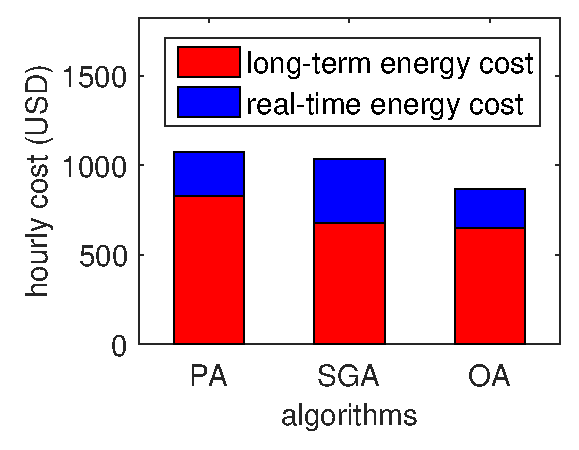
\includegraphics[width=.5\linewidth]{figs/cost_comparison_beta_0} 
		\label{fig:beta_0}}
	\subfloat[Vary $\beta$]{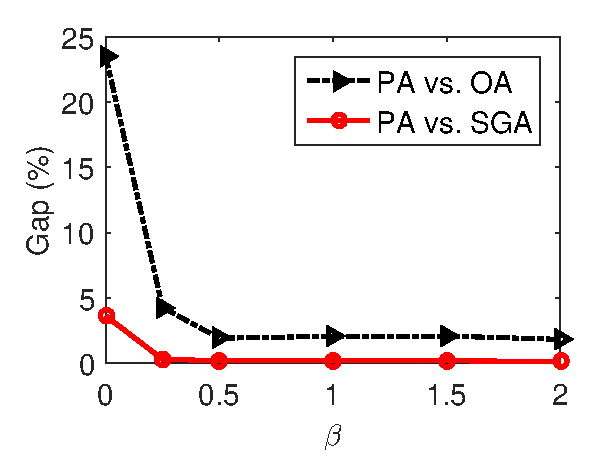
\includegraphics[width=.5\linewidth]{figs/vary_beta}
		\label{fig:vary_beta}}    
	\caption{The impact of delay on the proposed algorithms.}
	\label{fig:betas}
	\vspace{-0.3cm}
\end{figure}

\diff{\emph{How does the trade-off between energy costs and delay costs benefit our proposed algorithms?}
To answer this question, we vary the constant factor $\beta$ that weighs the delay costs relative to energy costs.
When $\beta=0$, i.e., the delay costs are ignored, the cost breakdown are shown in Figure \ref{fig:beta_0}. The performance gap between PA
and OA is 24\% that is much larger than the 2\% gap in Figure \ref{fig:cost_comparison} ($\beta=1$).
In this setting, SGA outperforms PA by 4\%. We observe that PA is more
aggressive compared to SGA in long-term procurement. Figure
\ref{fig:vary_beta} shows the performance gaps of PA versus OA and PA
versus SGA with varying $\beta.$ In this figure, the x-axis shows a
scaled $\beta,$ where a value of 1 corresponds to the default value.
We note that the performance gaps are significant when $\beta$ is
small ($<0.25$). However, the gaps are very small when $\beta$ is
relatively large ($\geq 0.5$).
}
%To show that GLB helps PA to perform well, we carry out another experiment assuming that there is only one single data center in our system. The performance comparison is in Figure \ref{fig:single_dc}

%SGA is proved to have optimal cost saving and robust to any prediction error correlations and a much wider range of objective functions. Therefore, it is usually worth using SGA for large-scale geo-distributed data center systems which cost billions of dollars a year.


\diff{\textbf{Sensitivity Analysis}. The capability of our proposed algorithms depends on multiple impact factors, such as the ratio of real-time price to long-term price, renewable penetration rates, and prediction errors.}
%Hence, it is necessary to study the impact of these impact factors on the proposed algorithms.

\begin{figure}[!ht]    
	\centering
	\vspace{-0.5cm}
	\subfloat[PA vs. OA]{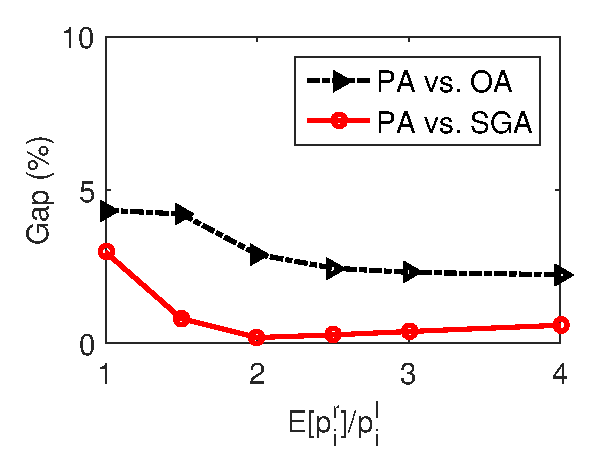
\includegraphics[width=.5\linewidth]{figs/vary_p_l_ratio}
		\label{fig:vary_p_l_ratio}}    
	\subfloat[Long term procurement]{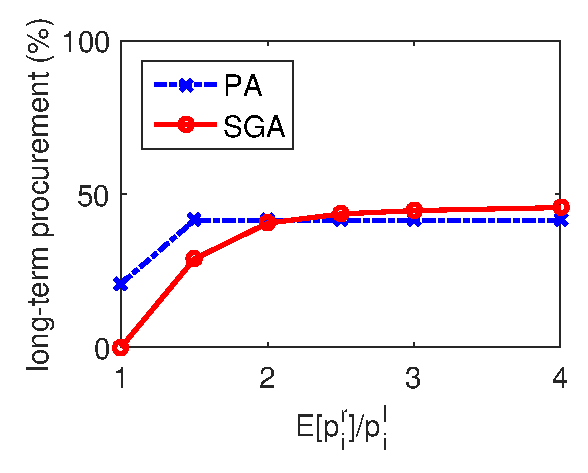
\includegraphics[width=.5\linewidth]{figs/vary_p_l_long_term_markets}
		\label{fig:vary_p_l_long_term_markets}}
	\vspace{-0.2cm}
	\caption{The impacts of long-term prices on the proposed algorithms. The gaps between the proposed algorithms and OA are small at various ratios of real-time prices to long-term prices.}
	\label{fig:prices}
	\vspace{-0.3cm}
\end{figure}

\emph{Impact of the ratio of real-time price to long-term price.} We carry out another study that quantifies the impact of the ratio of real-time prices to the long-term prices on our proposed algorithms as in Figure {\ref{fig:prices}}. In this experiment, the long term prices are fixed, and we scale the real-time prices. Figure {\ref{fig:vary_p_l_ratio}} shows the performance gaps of PA versus SGA and PA versus OA. In general, the gaps are small whatever the ratio is. Figure {\ref{fig:vary_p_l_long_term_markets}} illustrates the behaviors of PA and SGA in long-term markets. SGA is more conservative than PA when the ratio is small ($<2$). When the real-time prices are as cheap as the long-term prices, being more aggressive in long-term actually results in higher financial risk to the cloud providers. In contrast, SGA is more aggressive in long-term markets as the ratio becomes larger than 2.

\emph{Impact of renewable energy.} Renewable energy has been increasingly used to power data centers. Hence, we investigate the impacts of renewable energy integration on our energy procurement system. We scale the penetration levels of renewable energy from $5\%$ to $95\%$ of the total demand. We consider PV generation and wind generation as two main sources of renewable energy.

\begin{figure}[!ht]    
	\centering
	\vspace{-0.3cm}
	\subfloat[PV penetration]{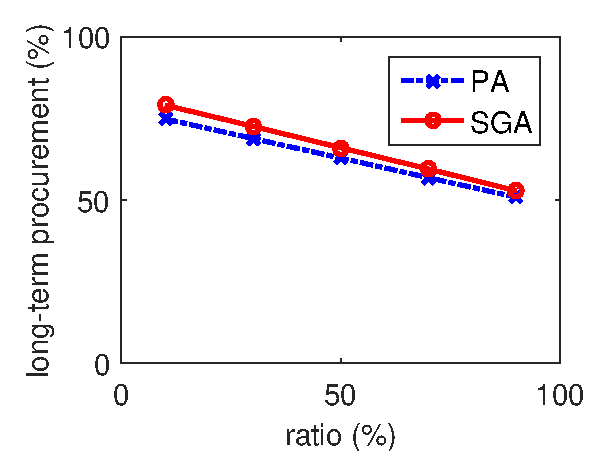
\includegraphics[width=.5\linewidth]{figs/solar_impact2}}
	\subfloat[Wind penetration]{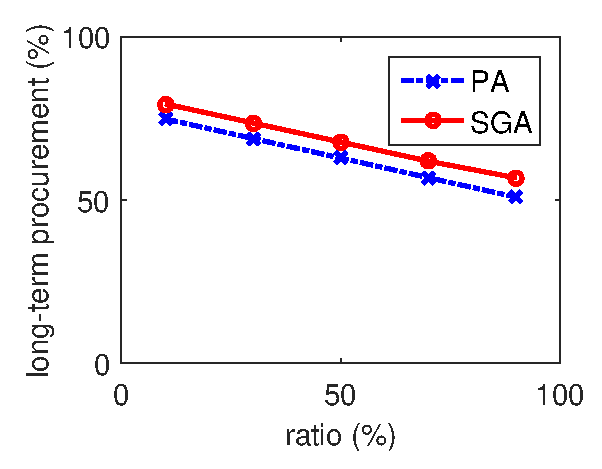
\includegraphics[width=.5\linewidth]{figs/wind_impact2}} 
	\vspace{-0.2cm}
	\caption{Impacts of renewable energy penetration levels on long-term energy procurement. SGA becomes less aggressive in the PV generation case than the wind generation case compared to PA.}
	\label{fig:renewableImpactLTEnergy}
	\vspace{-0.2cm}
\end{figure}

The impacts of renewable energy on the behaviors of PA and SGA are shown in Figure \ref{fig:renewableImpactLTEnergy}. Here, the x-axis represents the penetration levels of renewable energy, and the y-axis is the ratio (\%) of total electricity purchased in long-term markets. PA performs similarly in both cases because it is only based on the predicted values. However, SGA is closer to PA in the PV generation case as the penetration of renewable energy increases, yet becomes more aggressive than PA in the wind generation case. The reason lies in the error distributions in Figure \ref{fig:hourlyDistribution}. While the prediction errors of PV generation are concentrated on two peaks, the prediction errors of wind generation are centered around only one peak (around $-80\%$). 

%It means that wind generation allows SGA to find an optimal solution corresponding to the unique peak, but SGA has to find an optimal solution corresponding to a point between the two peaks.

%\subsection{How can the long-term forecaster impacts on SGA?} 

\emph{Impact of prediction errors.} So far, we have worked with the
empirical (or `real') prediction error distributions. We now study the
dependence of the distribution of prediction errors on the performance
of our procurement system.
%We obtained the prediction errors from AR methods. However, different prediction methods may give different error distributions. Furthermore, as the prediction range varies from days to years, the MAEs of prediction also increases. Thus, we continue to study the impacts of error distributions and MAEs.

\begin{figure}[!h]    
	\centering
	\vspace{-0.5cm}
	\subfloat[Error distributions ]{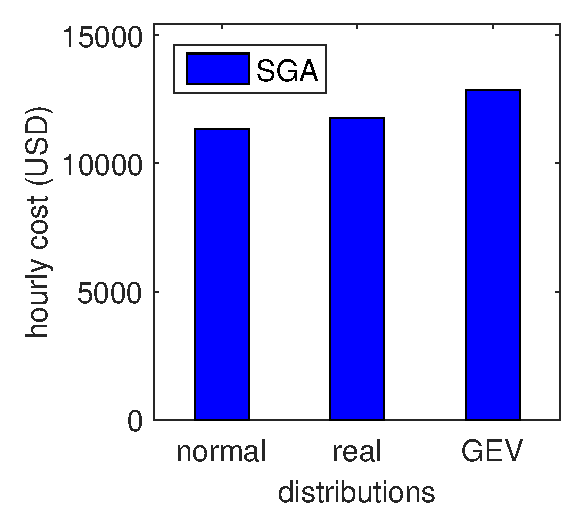
\includegraphics[width=.5\linewidth]{figs/distribution_impact}
		\label{fig:impactOfErrorDistribution_a}}
	\subfloat[Prediction errors ]{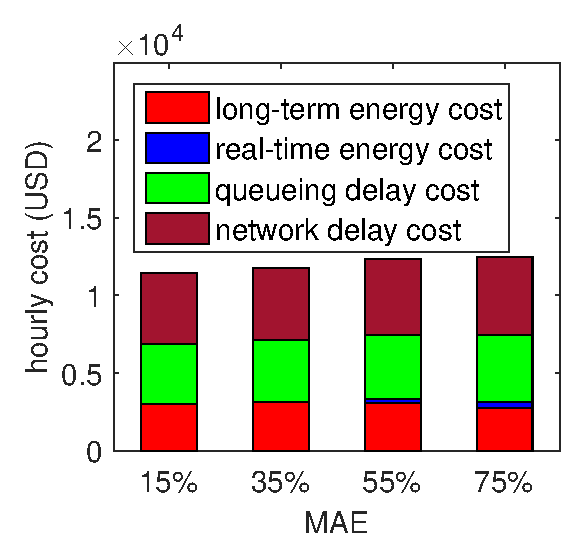
\includegraphics[width=.5\linewidth]{figs/rmse_impact}
		\label{fig:impactOfErrorDistribution_b}}  
	\vspace{-0.2cm}  
	\caption{Impacts of predictions on cost performance.}
	\label{fig:impactOfErrorDistribution}
	\vspace{-0.2cm}
\end{figure}

Figure \ref{fig:impactOfErrorDistribution_a} presents the cost of SGA under three different error distributions, i.e. normal, `real, and generalized extreme value (GEV)~\cite{corcoran2002modelling}. The normal distribution is symmetric around its mean. The GEV distribution is asymmetric and widely used in risk management and finance. We also consider the distribution of AR prediction errors as the `real' distribution. The MAEs of each are set at 35\% for fair comparison. Figure \ref{fig:impactOfErrorDistribution_a} shows that the cost using normal distribution is the best among three error distributions while GEV is the worst. %Similarly to previous case studies, PA also achieves very close performance to SGA. 

Figure \ref{fig:impactOfErrorDistribution_b} shows the cost of SGA with respect to different MAEs of `real' distribution.  As the prediction errors increase, the real-time cost (real-time energy cost and delay cost) increase to compensate for the mis-provisioning in long-term markets. Furthermore, the total cost increases by 10\% as the prediction errors increase from 15\% to 75\%. 

